% This template has been tested with IEEEtran of 2015.

% !TeX spellcheck = en-US
% LTeX: language=en-US
% !TeX encoding = utf8
% !TeX program = pdflatex
% !BIB program = bibtex
% -*- coding:utf-8 mod:LaTeX -*-

% DO NOT DOWNLOAD IEEEtran.cls - Use the one of your LaTeX distribution
% For the final version, replace "draftcls" by "final"
\documentclass[11pt, final, conference, letterpaper, twocolumn]{IEEEtran}[2015/08/26]

% Balance the last page
% The pbalance package (see https://ctan.org/pkg/pbalance) "just works" (in contrast to balance.sty or other solutions)
\usepackage{pbalance}

% backticks (`) are rendered as such in verbatim environments.
% See following links for details:
%   - https://tex.stackexchange.com/a/341057/9075
%   - https://tex.stackexchange.com/a/47451/9075
%   - https://tex.stackexchange.com/a/166791/9075
\usepackage{upquote}

% Set English as language and allow to write hyphenated"=words
%
% Even though `american`, `english` and `USenglish` are synonyms for babel package (according to https://tex.stackexchange.com/questions/12775/babel-english-american-usenglish), the llncs document class is prepared to avoid the overriding of certain names (such as "Abstract." -> "Abstract" or "Fig." -> "Figure") when using `english`, but not when using the other 2.
% english has to go last to set it as default language
\usepackage[ngerman,main=english]{babel}
%
% Hint by http://tex.stackexchange.com/a/321066/9075 -> enable "= as dashes
\addto\extrasenglish{\languageshorthands{ngerman}\useshorthands{"}}

% Links behave as they should. Enables "\url{...}" for URL typesettings.
% Allow URL breaks also at a hyphen, even though it might be confusing: Is the "-" part of the address or just a hyphen?
% See https://tex.stackexchange.com/a/3034/9075.
\usepackage[hyphens]{url}

% When activated, use text font as url font, not the monospaced one.
% For all options see https://tex.stackexchange.com/a/261435/9075.
% \urlstyle{same}

% Improve wrapping of URLs - hint by http://tex.stackexchange.com/a/10419/9075
\makeatletter
\g@addto@macro{\UrlBreaks}{\UrlOrds}
\makeatother

% nicer // - solution by http://tex.stackexchange.com/a/98470/9075
% DO NOT ACTIVATE -> prevents line breaks
%\makeatletter
%\def\Url@twoslashes{\mathchar`\/\@ifnextchar/{\kern-.2em}{}}
%\g@addto@macro\UrlSpecials{\do\/{\Url@twoslashes}}
%\makeatother


% use nicer font for code
\usepackage[zerostyle=b,scaled=.75]{newtxtt}

% Has to be loaded AFTER any font packages. See https://tex.stackexchange.com/a/2869/9075.
\usepackage[T1]{fontenc}

% Character protrusion and font expansion. See http://www.ctan.org/tex-archive/macros/latex/contrib/microtype/

\usepackage[
  babel=true, % Enable language-specific kerning. Take language-settings from the languge of the current document (see Section 6 of microtype.pdf)
  expansion=alltext,
  protrusion=alltext-nott, % Ensure that at listings, there is no change at the margin of the listing
  final % Always enable microtype, even if in draft mode. This helps finding bad boxes quickly.
        % In the standard configuration, this template is always in the final mode, so this option only makes a difference if "pros" use the draft mode
]{microtype}

% \texttt{test -- test} keeps the "--" as "--" (and does not convert it to an en dash)
\DisableLigatures{encoding = T1, family = tt* }

%\DeclareMicrotypeSet*[tracking]{my}{ font = */*/*/sc/* }%
%\SetTracking{ encoding = *, shape = sc }{ 45 }
% Source: http://homepage.ruhr-uni-bochum.de/Georg.Verweyen/pakete.html
% Deactiviated, because does not look good

\usepackage{graphicx}

% Diagonal lines in a table - http://tex.stackexchange.com/questions/17745/diagonal-lines-in-table-cell
% Slashbox is not available in texlive (due to licensing) and also gives bad results. Thus, we use diagbox
\usepackage{diagbox}

\usepackage{xcolor}

% Code Listings
\usepackage{listings}

\definecolor{eclipseStrings}{RGB}{42,0.0,255}
\definecolor{eclipseKeywords}{RGB}{127,0,85}
\colorlet{numb}{magenta!60!black}

% JSON definition
% Source: https://tex.stackexchange.com/a/433961/9075

\lstdefinelanguage{json}{
    basicstyle=\normalfont\ttfamily,
    commentstyle=\color{eclipseStrings}, % style of comment
    stringstyle=\color{eclipseKeywords}, % style of strings
    numbers=left,
    numberstyle=\scriptsize,
    stepnumber=1,
    numbersep=8pt,
    showstringspaces=false,
    breaklines=true,
    frame=lines,
    % backgroundcolor=\color{gray}, %only if you like
    string=[s]{"}{"},
    comment=[l]{:\ "},
    morecomment=[l]{:"},
    literate=
        *{0}{{{\color{numb}0}}}{1}
         {1}{{{\color{numb}1}}}{1}
         {2}{{{\color{numb}2}}}{1}
         {3}{{{\color{numb}3}}}{1}
         {4}{{{\color{numb}4}}}{1}
         {5}{{{\color{numb}5}}}{1}
         {6}{{{\color{numb}6}}}{1}
         {7}{{{\color{numb}7}}}{1}
         {8}{{{\color{numb}8}}}{1}
         {9}{{{\color{numb}9}}}{1}
}

\lstset{
  % everything between (* *) is a latex command
  escapeinside={(*}{*)},
  %
  language=json,
  %
  showstringspaces=false,
  %
  extendedchars=true,
  %
  basicstyle=\footnotesize\ttfamily,
  %
  commentstyle=\slshape,
  %
  % default: \rmfamily
  stringstyle=\ttfamily,
  %
  breaklines=true,
  %
  breakatwhitespace=true,
  %
  % alternative: fixed
  columns=flexible,
  %
  numbers=left,
  %
  numberstyle=\tiny,
  %
  basewidth=.5em,
  %
  xleftmargin=.5cm,
  %
  % aboveskip=0mm,
  %
  % belowskip=0mm,
  %
  captionpos=b
}

% Enable Umlauts when using \lstinputputlisting.
% See https://stackoverflow.com/a/29260603/873282 für details.
% listingsutf8 did not work in June 2020.
\lstset{literate=
  {á}{{\'a}}1 {é}{{\'e}}1 {í}{{\'i}}1 {ó}{{\'o}}1 {ú}{{\'u}}1
  {Á}{{\'A}}1 {É}{{\'E}}1 {Í}{{\'I}}1 {Ó}{{\'O}}1 {Ú}{{\'U}}1
  {à}{{\`a}}1 {è}{{\`e}}1 {ì}{{\`i}}1 {ò}{{\`o}}1 {ù}{{\`u}}1
  {À}{{\`A}}1 {È}{{\'E}}1 {Ì}{{\`I}}1 {Ò}{{\`O}}1 {Ù}{{\`U}}1
  {ä}{{\"a}}1 {ë}{{\"e}}1 {ï}{{\"i}}1 {ö}{{\"o}}1 {ü}{{\"u}}1
  {Ä}{{\"A}}1 {Ë}{{\"E}}1 {Ï}{{\"I}}1 {Ö}{{\"O}}1 {Ü}{{\"U}}1
  {â}{{\^a}}1 {ê}{{\^e}}1 {î}{{\^i}}1 {ô}{{\^o}}1 {û}{{\^u}}1
  {Â}{{\^A}}1 {Ê}{{\^E}}1 {Î}{{\^I}}1 {Ô}{{\^O}}1 {Û}{{\^U}}1
  {Ã}{{\~A}}1 {ã}{{\~a}}1 {Õ}{{\~O}}1 {õ}{{\~o}}1
  {œ}{{\oe}}1 {Œ}{{\OE}}1 {æ}{{\ae}}1 {Æ}{{\AE}}1 {ß}{{\ss}}1
  {ű}{{\H{u}}}1 {Ű}{{\H{U}}}1 {ő}{{\H{o}}}1 {Ő}{{\H{O}}}1
  {ç}{{\c c}}1 {Ç}{{\c C}}1 {ø}{{\o}}1 {å}{{\r a}}1 {Å}{{\r A}}1
}

% For easy quotations: \enquote{text}
% This package is very smart when nesting is applied, otherwise textcmds (see below) provides a shorter command
\usepackage[autostyle=true]{csquotes}

% Enable using "`quote"' - see https://tex.stackexchange.com/a/150954/9075
\defineshorthand{"`}{\openautoquote}
\defineshorthand{"'}{\closeautoquote}

% Nicer tables (\toprule, \midrule, \bottomrule)
\usepackage{booktabs}

% Extended enumerate, such as \begin{compactenum}
\usepackage{paralist}

% Bibliopgraphy enhancements
%  - enable \cite[prenote][]{ref}
%  - enable \cite{ref1,ref2}
% Alternative: \usepackage{cite}, which enables \cite{ref1, ref2} only (otherwise: Error message: "White space in argument")

% Doc: http://texdoc.net/natbib
\usepackage[%
  square,        % for square brackets
  comma,         % use commas as separators
  numbers,       % for numerical citations;
  %sort           % orders multiple citations into the sequence in which they appear in the list of references;
  sort&compress % as sort but in addition multiple numerical citations
                  % are compressed if possible (as 3-6, 15);
]{natbib}

% Same fontsize as without natbib
\renewcommand{\bibfont}{\normalfont\footnotesize}

% Enable hyperlinked author names in the case of \citet
% Source: https://tex.stackexchange.com/a/76075/9075
\usepackage{etoolbox}
\makeatletter
\patchcmd{\NAT@test}{\else \NAT@nm}{\else \NAT@hyper@{\NAT@nm}}{}{}
\makeatother

% Enable nice comments
\usepackage{pdfcomment}

\newcommand{\commentontext}[2]{\colorbox{yellow!60}{#1}\pdfcomment[color={0.234 0.867 0.211},hoffset=-6pt,voffset=10pt,opacity=0.5]{#2}}
\newcommand{\commentatside}[1]{\pdfcomment[color={0.045 0.278 0.643},icon=Note]{#1}}

% Compatibality with packages todo, easy-todo, todonotes
\newcommand{\todo}[1]{\commentatside{#1}}

% Compatiblity with package fixmetodonotes
\newcommand{\TODO}[1]{\commentatside{#1}}

% Put footnotes below floats
% Source: https://tex.stackexchange.com/a/32993/9075
\usepackage{stfloats}
\fnbelowfloat

\usepackage[group-minimum-digits=4,per-mode=fraction]{siunitx}
\addto\extrasgerman{\sisetup{locale = DE}}

% Enable that parameters of \cref{}, \ref{}, \cite{}, ... are linked so that a reader can click on the number an jump to the target in the document
\usepackage{hyperref}

% Enable hyperref without colors and without bookmarks
\hypersetup{
  hidelinks,
  colorlinks=true,
  allcolors=black,
  pdfstartview=Fit,
  breaklinks=true
}

% Enable correct jumping to figures when referencing
\usepackage[all]{hypcap}

\usepackage[caption=false,font=footnotesize]{subfig}

\usepackage[incolumn]{mindflow}

% Extensions for references inside the document (\cref{fig:sample}, ...)
% Enable usage \cref{...} and \Cref{...} instead of \ref: Type of reference included in the link
% That means, "Figure 5" is a full link instead of just "5".
\usepackage[capitalise,nameinlink,noabbrev]{cleveref}

\crefname{listing}{Listing}{Listings}
\Crefname{listing}{Listing}{Listings}
\crefname{lstlisting}{Listing}{Listings}
\Crefname{lstlisting}{Listing}{Listings}

\usepackage{lipsum}

% For demonstration purposes only
% These packages can be removed when all examples have been deleted
\usepackage[math]{blindtext}
\usepackage{mwe}
\usepackage[realmainfile]{currfile}
\usepackage{tcolorbox}
\tcbuselibrary{listings}

%introduce \powerset - hint by http://matheplanet.com/matheplanet/nuke/html/viewtopic.php?topic=136492&post_id=997377
\DeclareFontFamily{U}{MnSymbolC}{}
\DeclareSymbolFont{MnSyC}{U}{MnSymbolC}{m}{n}
\DeclareFontShape{U}{MnSymbolC}{m}{n}{
  <-6>    MnSymbolC5
  <6-7>   MnSymbolC6
  <7-8>   MnSymbolC7
  <8-9>   MnSymbolC8
  <9-10>  MnSymbolC9
  <10-12> MnSymbolC10
  <12->   MnSymbolC12%
}{}
\DeclareMathSymbol{\powerset}{\mathord}{MnSyC}{180}

\usepackage{xspace}
%\newcommand{\eg}{e.\,g.\xspace}
%\newcommand{\ie}{i.\,e.\xspace}
\newcommand{\eg}{e.\,g.,\ }
\newcommand{\ie}{i.\,e.,\ }

% Enable hyphenation at other places as the dash.
% Example: applicaiton\hydash specific
\makeatletter
\newcommand{\hydash}{\penalty\@M-\hskip\z@skip}
% Definition of "= taken from http://mirror.ctan.org/macros/latex/contrib/babel-contrib/german/ngermanb.dtx
\makeatother

% Add manual adapted hyphenation of English words
% See https://ctan.org/pkg/hyphenex and https://tex.stackexchange.com/a/22892/9075 for details
% Does not work on MiKTeX, therefore disabled - issue reported at https://github.com/MiKTeX/miktex-packaging/issues/271
% \input{ushyphex}

% correct bad hyphenation here
%\hyphenation{op-tical net-works semi-conduc-tor}

% Enable copy and paste of text from the PDF
% Only required for pdflatex. It "just works" in the case of lualatex.
% Alternative: cmap or mmap package
% mmap enables mathematical symbols, but does not work with the newtx font set
% See: https://tex.stackexchange.com/a/64457/9075
% Other solutions outlined at http://goemonx.blogspot.de/2012/01/pdflatex-ligaturen-und-copynpaste.html and http://tex.stackexchange.com/questions/4397/make-ligatures-in-linux-libertine-copyable-and-searchable
% Trouble shooting outlined at https://tex.stackexchange.com/a/100618/9075
%
% According to https://tex.stackexchange.com/q/451235/9075 this is the way to go
\input glyphtounicode
\pdfgentounicode=1

\begin{document}
% Enable following command if you need to typeset "IEEEpubid".
% See https://bytefreaks.net/tag/ieeeoverridecommandlockouts for details.
%\IEEEoverridecommandlockouts

\title{Vitis Flow and Design Exploration on Alveo U280 FPGA Board}

\author{%
  \IEEEauthorblockN{Pablo Lopez, Zephram Tripp}
  \IEEEauthorblockA{Brigham Young University, EcEn 625}
}

% use for special paper notices
%\IEEEspecialpapernotice{(Invited Paper)}

% make the title area
\maketitle

% In case you want to add a copyright statement.
% Works only in the compsoc conference mode.
%
% Source: https://tex.stackexchange.com/a/325013/9075
%
% All possible solutions:
%  - https://tex.stackexchange.com/a/325013/9075
%  - https://tex.stackexchange.com/a/279134/9075
%  - https://tex.stackexchange.com/q/279789/9075 (TikZ)
%  - https://tex.stackexchange.com/a/200330/9075 - for non-compsocc papers
\iffalse
  \IEEEoverridecommandlockouts
  \IEEEpubid{\begin{minipage}{\textwidth}\ \\[12pt] \centering
      1551-3203 \copyright 2015 IEEE.
      Personal use is permitted, but republication/redistribution requires IEEE permission.
      \\
      See \url{https://www.ieee.org/publications_standards/publications/rights/index.html} for more information.
    \end{minipage}}
\fi

% \begin{abstract}
% %\lipsum[1]
% \end{abstract}

% For peer review papers, you can put extra information on the cover
% page as needed:
% \ifCLASSOPTIONpeerreview
% \begin{center} \bfseries EDICS Category: 3-BBND \end{center}
% \fi
%
% For peerreview papers, this IEEEtran command inserts a page break and
% creates the second title. It will be ignored for other modes.
%\IEEEpeerreviewmaketitle

\section{Introduction}
\label{sec:introduction}

As hardware designs become more complex, and the allure of hardware acceleration on platforms like field-programmable gate arrays (FPGAs) becomes more attractive to corporations and others seeking to maximize the performance of their algorithms, it becomes necessary for tools to be developed that allow for more effective use of hardware acceleration. One of the tools used in this regard is Vitis HLS, Xilinx's proprietary high-level synthesis tool, which uses C++ code along with a few simple preprocessor directives called pragmas to create hardware designs on a higher, more conceptual level. In order to better facilitate high-level synthesis of hardware designs, Xilinx developed an additional flow target for the Vitis HLS tool called the Vitis Kernel Flow.
Our first goal for our project was to explore this new flow and compare its performance with the Vivado IP flow when they are used to implement a simple knn algorithm.
The second goal was to explore different memory implementations of this algorithm using the resources found in the Xilinx Alveo U280 Data Center Accelerator Card.

\section{knn Algorithm}
\label{sec:knn-algorithm}

The algorithm we chose to implement for this project was the \textit{k}-nearest neighbors algorithm for image recognition, as depicted in figure \ref{fig:ex:knn}. To prepare the test set, images of each item to identify are scanned, identified, and each pixel is converted to a 0 or a 1. Each tested image is processed in the same way. We used the training and test data from labs 4 and 5. For these labs, we used the \textit{k}-nearest neighbors algorithm to identify images of the Hindu-Arabic numerals 0-9. For a particular test case, it is compared against each image in the data set to find the lowest Hamming distances between images, until we find the \textit{k} smallest Hamming distances between images for each numeral. Then from among these 10\textit{k} items, the lowest \textit{k} elements become the voters that decide what the result should be, with ties being broken arbitrarily. The algorithm we used had an accuracy of 86\% for the test data set when implemented in software, and an 89\% accuracy when implemented in hardware. Our goal was not to optimize this accuracy, but to test the performance of the algorithm with several different implementations.

\begin{figure}
  \centering
  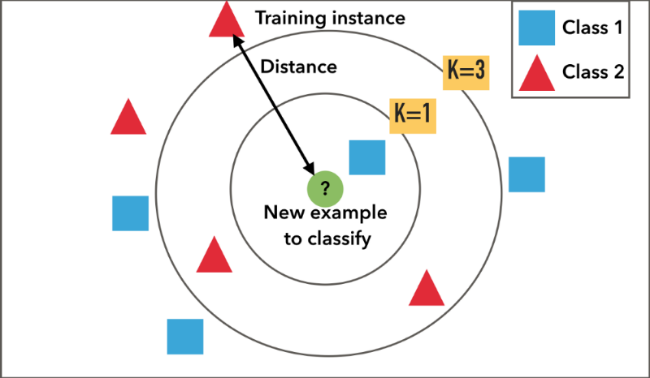
\includegraphics[width=.75\linewidth]{knearestneighbors.png}
  \caption{Example of knn algorithm with all elements within a circle representing the voters at that value of k for the test object (green)}
  \label{fig:ex:knn}
\end{figure}


\section{Approaches}
\label{sec:approaches}

To implement the \textit{k}-nearest neighbors algorithm on the board and accelerate it, we needed to use Vitis HLS. Vitis HLS offers two design flows for users, and we were excited to try them both out.

\subsection{Vitis Kernel Flow}

\begin{figure}
  \centering
  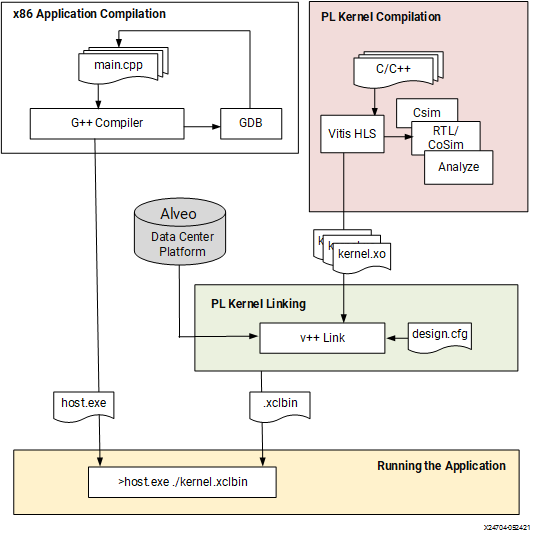
\includegraphics[width=.75\linewidth]{vitiskernelflow.png}
  \caption{Diagram of the Vitis Kernel Flow, from Xilinx}
  \label{fig:ex:vitiskernelflow}
\end{figure}

The approach we most wanted to explore for this project was the Vitis Kernel Flow. The documentation surrounding this new flow is scattered at best, but we did our best to try and find how to use it properly.

According to the documentation maintained by Xilinx, the goal of the Vitis Kernel Flow is to offer the opportunity for FPGAs to be reconfigured similarly to the kernels of a GPU. When using the Xilinx Kernel Flow, you first install a platform onto the board that serves as the base for kernel implementation. The platform we used was specific to the Alveo board, and we obtained it from Xilinx's website. Derived from this platform is a Xilinx Executable Binary file, which serves as the executable for the FPGA. The kernel is then linked into this executable at the time it is written to the board, so this effectively replaces the normal bitstream that would be programmed to the board. The kernels you write for the Vitis Kernel Flow must meet a few requirements as described in Xilinx's documentation. All Xilinx Runtime managed kernels must have at least one clock input and at least one slave Advanced eXtensible Interface Lite (AXI4-Lite) port, and there are required control registers as well. However, almost all of these requirements can be optional if you choose to create a user-managed kernel. However, you must then choose how to start and stop the kernel yourself. We decided to try to create an XRT-managed kernel for this project.

The Xilinx Runtime Library or XRT is a combination of Linux kernel drivers and userspace code that allows a host machine to communicated over PCIe with the FPGA board. This allows for easy control of the platform and the kernels added to it. This was one of the more complex parts of our project to use, as we did not realize we would need to install kernel drivers on our Linux machine in order to use the Vitis Kernel Flow. After we had installed these drivers, we ended up having to have our machine run with Secure Boot disabled in order to allow all of Xilinx's custom kernel drivers to work. After installing all these kernel drivers and the rest of the XRT, we were able to install the platform onto the Alveo board. We were then able to run all the verification tests provided in that code to prove the flow was working correctly. After this point, we attempted to create our own kernel, implementing the \textit{k}-nearest neighbors algorithm. Once we created the Xilinx Kernel file from Vitis HLS, we learned that we would need a host-side C++ program that would control the kernel. We wrote a quick host application, and ran it on the Alveo board, to no avail. After trying several other methods, we moved on to exploring other methods of using the Alveo board for the knn algorithm.

\subsection{Vivado IP Flow}

\begin{figure}
  \centering
  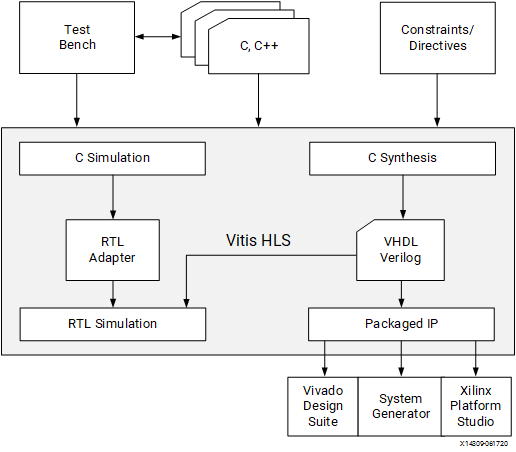
\includegraphics[width=.75\linewidth]{vivadoipflow.png}
  \caption{Diagram of the Vivado IP Flow, from Xilinx}
  \label{fig:ex:vivadoipflow}
\end{figure}

The Vivado IP Flow functions differently from the Vitis Kernel Flow. Instead of creating a Xilinx Kernel file, Vitis HLS creates a new Vivado block IP, which can be used in Vivado hardware designs. Once the block design is created in Vivado, it can be exported as a Xilinx Support Archive file, which can be imported into Vitis IDE to become a hardware platform with the proper functions to control the hardware. This hardware platform is then paired with an application written in C++ that runs on that platform. The application platform is then built and executed on the FPGA board.

For the Vivado IP Flow, we explored six different designs:

\subsubsection{Software}

For the software design of this algorithm, we decided to use the MicroBlaze soft processor core for its implementation.
Given the size of both the training and testing data, the auto-generated SOC using this core and its BRAMs could not handle the size of the data.
A new design using the board's DRAM became necessary.

\subsubsection{Software + DRAM}

The software design using the board's DRAM was able to successfully handle the size of the training and testing data.
It achieved an accuracy of 86\% on the test data set and when compiled using an O3 optimization, it was able to achieve a 2.21x speedup compared to the original design. The unoptimized software implementation became our baseline for all our future tests, so all speedup numbers are in comparison to the unoptimized software running on the MicroBlaze processor.

\subsubsection{Software + HBM}

For the software design using the HBM, due to time constraints and technical struggles, the implementation of this algorithm was not successfully completed. We were able to explore creating hardware designs using the high-bandwidth memory, but we were unable to discern how to have the DRAM and HBM work in concert with the MicroBlaze to get all the data in the right places at the right times. This could be a further exploration of our work in the future.

\subsubsection{Hardware}

After trying our best at software implementations, we wanted to move on to hardware accelerated implementations. We were able to create a hardware implementation that ran on the Alveo board using only flip-flops and lookup tables to store the training and test data. With this implementation, we got extremely good performance with an increased accuracy of 89\% and a more than 150,000 times speedup compared to the unoptimized software implementation.

\subsubsection{Hardware + DRAM}

With the hardware accelerated version working, we wanted to try and use the DRAM on the board as the interface for the arrays of data used by the algorithm. We successfully implemented this to a performance that was generally worse than pure flip-flops and lookup tables but still significantly better than the software implementation. We got a accuracy of 89\% and a speedup of more than 18,000 times compared to the unoptimized software implementation.

\subsubsection{Hardware + HBM}

For the hardware design of this algorithm using the HBM, again due to time constraints and technical challenges, the implementation of this algorithm was also not succesfully completed. We did explore this possibility as with the software implementation, but the documentation for the high bandwidth memory mostly focuses on the Vitis Kernel Flow, so it was difficult to find resources for solving our problems.

\section{Results}
\label{sec:results}

As we were never able to figure out the Vitis Kernel Flow, we were not able to get any results from that flow. However, we were able to get results from three of our six planned Vivado IP implementations. In the table, we additionally have a row showing the performance of optimized software, as optimized by the GNU C compiler (gcc) using the O3 optimization flag.

\begin{figure}
  \centering
  \begin{tabular}{c|ccc}
    \toprule
    Method       & Accuracy & Cycles  & Speedup \\
    \midrule
    SW + DRAM    & 86\%     & 2.92e11 & 1x      \\
    Optimized SW & 86\%     & 1.32e11 & 2.21x   \\
    Hardware     & 89\%     & 1.88e6  & 155090x \\
    HW + DRAM    & 89\%     & 1.62e7  & 18076x  \\
    \bottomrule
  \end{tabular}
  \caption{Results of Vivado IP Flow}
  \label{tab:ex:cref}
\end{figure}

\section{Conclusion}
\label{sec:conclusion}

After spending more than twenty hours trying to make the Vitis Kernel Flow work, we threw in the towel and moved on to working on the Vivado IP flow. Near the end of the project, we were able to find more documentation on using the Vitis Kernel Flow that, if we had found it earlier, we would hopefully have been more successful in this particular effort.
We came to understand that the Vitis Kernel Flow is convenient once it works, the problem is getting it to work. It seems as though the Vitis flow offers greater plug-and-play capabilities for people experienced in the design of software kernels, while avoiding the use of Vivado IP integrator and abstracting away the complexities of hardware, but reducing the freedom of the designer with respect to these complexities.
The installation guides for these tools could have been more clear and updated, and that would have been an additional boon to our project. As is, we cannot recommend the Vitis Kernel Flow to anyone inexperienced in the complexities of Linux kernel drivers and the design of GPU kernels, especially if the individual already has experience with hardware design flows.

In terms of memory exploration, we were also unable to use the high-bandwidth memory on the Alveo board. We would have liked to compare its performance to the performance of the DRAM on the same board. All the same, we were able to show, as in lab 5, that the transfer of data from memory to processor can often be the greatest roadblock to algorithm performance. We also showed that a pure software implementation was significantly worse than a hardware implementation when it comes to FPGA design.

All in all, we would recommend users of either of these flows to consider carefully what level of control they want over their design, as well as their experience with the relevant tools while making decisions on which of these flows to use. We hope that as the Vitis Kernel Flow becomes more common, it will have better documentation and guides to its use. We do continue to recommend that people seeking great algorithm performance turn to hardware acceleration as an effective way to find greater performance.

% Required for proper example rendering in the compiled PDF
% \newcount\LTGbeginlineexample
% \newcount\LTGendlineexample
% \newenvironment{ltgexample}%
% {\LTGbeginlineexample=\numexpr\inputlineno+1\relax}%
% {\LTGendlineexample=\numexpr\inputlineno-1\relax%
% %
% \tcbinputlisting{%
%   listing only,
%   listing file=\currfilepath,
%   colback=green!5!white,
%   colframe=green!25,
%   coltitle=black!90,
%   coltext=black!90,
%   left=8mm,
%   title=Corresponding \LaTeX{} code of \texttt{\currfilepath},
%   listing options={%
%     frame=none,
%     language={[LaTeX]TeX},
%     escapeinside={},
%     firstline=\the\LTGbeginlineexample,
%     lastline=\the\LTGendlineexample,
%     firstnumber=\the\LTGbeginlineexample,
%     basewidth=.5em,
%     aboveskip=0mm,
%     belowskip=0mm,
%     numbers=left,
%     xleftmargin=0mm,
%     numberstyle=\tiny,
%     numbersep=8pt%
%   }
% }
% }%

%This section contains hints on writing LaTeX.
%It focuses on minimal examples, which can be directly adapted to the content

%\subsection{Handling of paragraphs}

%\begin{ltgexample}
%One sentence per line.
% This rule is important for the usage of version control systems.
% A new line is generated with a blank line.
% As you would do in Word:
% New paragraphs are generated by pressing enter.
% In LaTeX, this does not lead to a new paragraph as LaTeX joins subsequent lines.
% In case you want a new paragraph, just press enter twice (!).
% This leads to an empty line.
% In word, there is the functionality to press shift and enter.
% This leads to a hard line break.
% The text starts at the beginning of a new line.
% In LaTeX, you can do that by using two backslashes (\textbackslash\textbackslash).\\
% This is rarely used.

% Please do \textit{not} use two backslashes for new paragraphs.
% For instance, this sentence belongs to the same paragraph, whereas the last one started a new one.
% A long motivation for that is provided at \url{http://loopspace.mathforge.org/HowDidIDoThat/TeX/VCS/#section.3}.
% \end{ltgexample}

% \subsection{Notes separated from the text}

% The package mindflow enables writing down notes and annotations in a way so that they are separated from the main text.

% \begin{ltgexample}
% \begin{mindflow}
% This is a small note.
% \end{mindflow}
% \end{ltgexample}

% \subsection{Hyphenation}

% \LaTeX{} automatically hyphenates words.
% When using microtype, there should be less hypnetations than in other settings.
% It might be necessary to tweak the hyphenations nevertheless.
% Here are some hints:

% \begin{ltgexample}
% In case you write \enquote{application-specific}, then the word will only be hyphenated at the dash.
% You can also write \verb1applica\allowbreak{}tion-specific1 (result: applica\allowbreak{}tion-specific), but this is much more effort.

% You can now write words containing hyphens which are hyphenated at other places in the word.
% For instance, \verb1application"=specific1 gets application"=specific.
% This is enabled by an additional configuration of the babel package.
% \end{ltgexample}

% \subsection{Typesetting Units}

% \begin{ltgexample}
% Numbers can written plain text (such as 100), by using the siunitx package like that:
% \SI{100}{\km\per\hour},
% or by using plain \LaTeX{} (and math mode):
% $100 \frac{\mathit{km}}{h}$.
% \end{ltgexample}

% \begin{ltgexample}
% \SI{5}{\percent} of \SI{10}{kg}
% \end{ltgexample}

% \begin{ltgexample}
% Numbers are automatically grouped: \num{123456}.
% \end{ltgexample}

% \subsection{Surrounding Text by Quotes}

% \begin{ltgexample}
% Please use the \enquote{enquote command} to quote something.
% Quoting with "`quote"' or ``quote'' also works.

% \end{ltgexample}

% \subsection{Cleveref examples}
% \label{sec:ex:cref}

% Cleveref demonstration: Cref at beginning of sentence, cref in all other cases.

% \begin{figure}
%     \centering
%     \includegraphics[width=.75\linewidth]{example-image-a}
%     \caption{Example figure for cref demo}
%     \label{fig:ex:cref}
% \end{figure}

% \begin{figure}
%     \centering
%     \begin{tabular}{ll}
%       \toprule
%       Heading1 & Heading2 \\
%       \midrule
%       One      & Two      \\
%       Thee     & Four     \\
%       \bottomrule
%     \end{tabular}
%     \caption{Example table for cref demo}
%     \label{tab:ex:cref}
% \end{figure}

% \begin{ltgexample}
% \Cref{fig:ex:cref} shows a simple fact, although \cref{fig:ex:cref} could also show something else.

% \Cref{tab:ex:cref} shows a simple fact, although \cref{tab:ex:cref} could also show something else.

% \Cref{sec:ex:cref} shows a simple fact, although \cref{sec:ex:cref} could also show something else.
% \end{ltgexample}

% \subsection{Figures}

% \begin{ltgexample}
% \Cref{fig:label} shows something interesting.

% \begin{figure}
%   \centering
%   \includegraphics[width=.8\linewidth]{example-image-golden}
%   \caption[Simple Figure]{Simple Figure. Based on \citet{mwe}.}
%   \label{fig:label}
% \end{figure}
% \end{ltgexample}


% One can span a figure across multiple columns by using \verb+\begin{figure*}+.
% See \cref{fig:16x9} as an example.

% \begin{ltgexample}
% \begin{figure*}
%   \centering
%   % note that \textwidth is used instead of \linewidth
%   % This ensures that the graphics width is 60% of the "page" (text block), and not just 60% of the current text column
%   % See https://tex.stackexchange.com/a/17085/9075 for details
%   \includegraphics[width=.6\textwidth]{example-image-16x9}
%   \caption{16x9 Figure}
%   \label{fig:16x9}
% \end{figure*}
% \end{ltgexample}


% \subsection{Sub Figures}

% An example of two sub figures is shown in \cref{fig:two_sub_figures}.

% \begin{ltgexample}
% \begin{figure*}[!b]
%     \centering
%     \subfloat[Case I]{\includegraphics[width=.4\linewidth]{example-image-a}%
%     \label{fig:first_case}}
%   \hfil
%     \subfloat[Case II]{\includegraphics[width=.4\linewidth]{example-image-b}%
%     \label{fig:second_case}}
%   \caption{Example figure with two sub figures.}
%   \label{fig:two_sub_figures}
% \end{figure*}
% \end{ltgexample}

% Note that often IEEE papers with subfigures do not employ subfigure
% captions (using the optional argument to \verb+\subfloat[]+), but instead will
% reference/describe all of them (a), (b), etc., within the main caption.
% Be aware that for subfig.sty to generate the (a), (b), etc., subfigure
% labels, the optional argument to \verb+\subfloat+ must be present. If a
% subcaption is not desired, just leave its contents blank,
% e.g., \verb+\subfloat[]+.
% An example is shown in \cref{fig:two_sub_figures_ieee}.

% \begin{ltgexample}
% \begin{figure*}[!b]
%     \centering
%     \subfloat[]{\includegraphics[width=.4\linewidth]{example-image-a}%
%     \label{fig:first_case_ieee}}
%   \hfil
%     \subfloat[]{\includegraphics[width=.4\linewidth]{example-image-b}%
%     \label{fig:second_case_ieee}}
%   \caption{Example figure with two sub figures. IEEE style. (a) The first case. (b) The second case.}
%   \label{fig:two_sub_figures_ieee}
% \end{figure*}
% \end{ltgexample}

% \subsection{Tables}

% Note that IEEE does not support \verb+\begin{table}+, one has to use \verb+\begin{figure}+.

% \begin{ltgexample}
% \begin{figure}
%   \caption{Simple Table}
%   \label{tab:simple}
%   \centering
%   \begin{tabular}{ll}
%     \toprule
%     Heading1 & Heading2 \\
%     \midrule
%     One      & Two      \\
%     Thee     & Four     \\
%     \bottomrule
%   \end{tabular}
% \end{figure}
% \end{ltgexample}

% \begin{ltgexample}
% % Source: https://tex.stackexchange.com/a/468994/9075
% \begin{figure}
% \caption{Table with diagonal line}
% \label{tab:diag}
% \begin{center}
% \begin{tabular}{|l|c|c|}
% \hline
% \diagbox[width=10em]{Diag\\Column Head I}{Diag Column\\Head II} & Second & Third \\
% \hline
% & foo & bar \\
% \hline
% \end{tabular}
% \end{center}
% \end{figure}
% \end{ltgexample}


% \subsection{Source Code}

% \begin{ltgexample}
% \Cref{lst:XML} shows source code written in XML.
% \Cref{line:comment} contains a comment.

% \begin{lstlisting}[
%   language=XML,
%   caption={Example XML Listing},
%   label={lst:XML}]
% <listing name="example">
%   <!-- comment --> (* \label{line:comment} *)
%   <content>not interesting</content>
% </listing>
% \end{lstlisting}
% \end{ltgexample}

% One can also add \verb+float+ as parameter to have the listing floating.
% \Cref{lst:flXML} shows the floating listing.

% \begin{ltgexample}
% \begin{lstlisting}[
%   % one can adjust spacing here if required
%   % aboveskip=2.5\baselineskip,
%   % belowskip=-.8\baselineskip,
%   float,
%   language=XML,
%   caption={Example XML listing -- placed as floating figure},
%   label={lst:flXML}]
% <listing name="example">
%   Floating
% </listing>
% \end{lstlisting}
% \end{ltgexample}

% One can also typeset JSON as shown in \cref{lst:json}.

% \begin{ltgexample}
% \begin{lstlisting}[
%   float,
%   language=json,
%   caption={Example JSON listing -- placed as floating figure},
%   label={lst:json}]
% {
%   key: "value"
% }
% \end{lstlisting}
% \end{ltgexample}

% Java is also possible as shown in \cref{lst:java}.

% \begin{ltgexample}
% \begin{lstlisting}[
%   caption={Example Java listing},
%   label=lst:java,
%   language=Java,
%   float]
% public class Hello {
%     public static void main (String[] args) {
%         System.out.println("Hello World!");
%     }
% }
% \end{lstlisting}
% \end{ltgexample}

% \subsection{Itemization}

% One can list items as follows:

% \begin{ltgexample}
% \begin{itemize}
% \item Item One
% \item Item Two
% \end{itemize}
% \end{ltgexample}

% With the package paralist, one can create itemizations with lesser spacing:

% \begin{ltgexample}
% \begin{compactitem}
% \item Item One
% \item Item Two
% \end{compactitem}
% \end{ltgexample}

% One can enumerate items as follows:

% \begin{ltgexample}
% \begin{enumerate}
%   \item Item One
%   \item Item Two
% \end{enumerate}
% \end{ltgexample}

% With the package paralist, one can create enumerations with lesser spacing:

% \begin{ltgexample}
% \begin{compactenum}
%   \item Item One
%   \item Item Two
% \end{compactenum}
% \end{ltgexample}

% With paralist, one can even have all items typset after each other and have them clean in the tex document:

% \begin{ltgexample}
% \begin{inparaenum}
%   \item All these items...
%   \item ...appear in one line
%   \item This is enabled by the paralist package.
% \end{inparaenum}
% \end{ltgexample}

% \subsection{Other Features}

% \begin{ltgexample}
% The words \enquote{workflow} and \enquote{dwarflike} can be copied from the PDF and pasted to a text file.
% \end{ltgexample}

% \begin{ltgexample}
% The symbol for powerset is now correct: $\powerset$ and not a Weierstrass p ($\wp$).

% $\powerset({1,2,3})$
% \end{ltgexample}

% \begin{ltgexample}
% Brackets work as designed:
% <test>
% One can also input backquotes in verbatim text: \verb|`test`|.
% \end{ltgexample}


% \section{Conclusion and Outlook}
% \label{sec:outlook}
% \lipsum[1-2]

% % regular IEEE prefers the singular form
% \section*{Acknowledgment}

% Identification of funding sources and other support, and thanks to individuals and groups that assisted in the research and the preparation of the work should be included in an acknowledgment section, which is placed just before the reference section in your document \cite{acmart}.

% %%% ===============================================================================
% %%% Bibliography
% %%% ===============================================================================

% In the bibliography, use \texttt{\textbackslash textsuperscript} for \enquote{st}, \enquote{nd}, \ldots:
% E.g., \enquote{The 2\textsuperscript{nd} conference on examples}.
% When you use \href{https://www.jabref.org}{JabRef}, you can use the clean up command to achieve that.
% See \url{https://help.jabref.org/en/CleanupEntries} for an overview of the cleanup functionality.

% % trigger a \newpage just before the given reference
% % number - used to balance the columns on the last page
% % adjust value as needed - may need to be readjusted if
% % the document is modified later
% %\IEEEtriggeratref{8}
% % The "triggered" command can be changed if desired:
% %\IEEEtriggercmd{\enlargethispage{-5in}}

% % Enable to reduce spacing between bibitems (source: https://tex.stackexchange.com/a/25774)
% % \def\IEEEbibitemsep{0pt plus .5pt}

% \bibliographystyle{IEEEtranN} % IEEEtranN is the natbib compatible bst file
% % argument is your BibTeX string definitions and bibliography database(s)
% \bibliography{paper}

% % Enfore empty line after bibliography
% \ \\
% %
% All links were last followed on October 5, 2020.

\end{document}